% arara: makeindex

% Template for IEEE papers
%% bare_conf.tex
%% V1.4b
%% 2015/08/26
%% by Michael Shell
%% See:
%% http://www.michaelshell.org/
%% for current contact information.
%%
%% This is a skeleton file demonstrating the use of IEEEtran.cls
%% (requires IEEEtran.cls version 1.8b or later) with an IEEE
%% conference paper.
%%
%% Support sites:
%% http://www.michaelshell.org/tex/ieeetran/
%% http://www.ctan.org/pkg/ieeetran
%% and
%% http://www.ieee.org/

%%*************************************************************************
%% Legal Notice:
%% This code is offered as-is without any warranty either expressed or
%% implied; without even the implied warranty of MERCHANTABILITY or
%% FITNESS FOR A PARTICULAR PURPOSE! 
%% User assumes all risk.
%% In no event shall the IEEE or any contributor to this code be liable for
%% any damages or losses, including, but not limited to, incidental,
%% consequential, or any other damages, resulting from the use or misuse
%% of any information contained here.
%%
%% All comments are the opinions of their respective authors and are not
%% necessarily endorsed by the IEEE.
%%
%% This work is distributed under the LaTeX Project Public License (LPPL)
%% ( http://www.latex-project.org/ ) version 1.3, and may be freely used,
%% distributed and modified. A copy of the LPPL, version 1.3, is included
%% in the base LaTeX documentation of all distributions of LaTeX released
%% 2003/12/01 or later.
%% Retain all contribution notices and credits.
%% ** Modified files should be clearly indicated as such, including  **
%% ** renaming them and changing author support contact information. **
%%*************************************************************************


% *** Authors should verify (and, if needed, correct) their LaTeX system  ***
% *** with the testflow diagnostic prior to trusting their LaTeX platform ***
% *** with production work. The IEEE's font choices and paper sizes can   ***
% *** trigger bugs that do not appear when using other class files.       ***                          ***
% The testflow support page is at:
% http://www.michaelshell.org/tex/testflow/

\documentclass{book}
% \def\nolinkurl{\url}
%\usepackage{nohyperref}
% \def\UrlBreaks{\do\/\do-}
\usepackage[table,xcdraw,dvipsnames]{xcolor} % Used by spritegrid and others.
\usepackage[obeyspaces,spaces]{url}
\usepackage{arydshln}
\usepackage{booktabs}
\usepackage{hyperref}
\usepackage{afterpage}
%\usepackage{xcolor}

%\usepackage{breakurl}
\usepackage{flushend}
\usepackage[toc,page]{appendix}
\usepackage{parskip}
\usepackage{graphicx} % Used by spritegrid and others.
\usepackage{tikzpagenodes}
\usepackage{imakeidx}
\usepackage[raggedright]{titlesec}
\usepackage{aeb-minitoc}
\usepackage{fix-cm}
\usepackage{textpos}

% For Mega65 key display
% This is a `keys' element for displaying a Mega65 keyboard key
% using a black filled label with rounded edges.
% In order to display a key as a title, use:
%
%     \megakey[title]{Run/Stop}
%
% For displaying a key as a part of the normal document flow, simply use:
%
%    \megakey{Shift}
%
%
% If you get warnings on special characters, mathematical characters etc, use $, eg:
%
%    \megakey{$\leftarrow$}
%
% Other sizes are supported, as part of tcolorbox:
% http://mirror.aarnet.edu.au/pub/CTAN/macros/latex/contrib/tcolorbox/tcolorbox.pdf#subsubsection.4.7.5 however, only `title' and the default: `small' are proposed for use in this manual.
%
% The second macro available here is the megasymbolkey.
% This will display the MEGA symbol as white on a black key box. Simply use:
%
%		 \megasymbolkey
%

\usepackage{tcolorbox}

\newtcbox{\megakeyinner}[1][small]{colback=black, coltext=white, size=#1, fontupper=\bfseries, nobeforeafter,box align=bottom,baseline=3pt,text height=7pt}
\newcommand{\megakey}[2][small]{\megakeyinner[#1]{\uppercase{#2}}}

\newtcbox{\megasymbolkeyinner}{colback=black, coltext=white, clip title=false. fontupper=\symbolfont, box align=bottom,baseline=3pt,text height=7pt}
\newcommand{\megasymbolkey}{\megakeyinner{\megasymbol[white]}\ }


% For Mega65 display of code, listings and screen activity
% This is an element for displaying output from the Mega65 screen.
% It can display program code or to show activity on the screen.
% Example of use:
%
%    \begin{screenoutput}
%    10 OPEN 1,8,0,"$0:*,P,R
%    20 : IF DS THEN PRINT DS$: GOTO 100
%    30 GET#1,X$,X$
%    40 DO
%    50 : GET#1,X$,X$: IF ST THEN EXIT
%    60 : GET#1,BL$,BH$
%    70 : LINE INPUT#1, F$
%    80 : PRINT LEFT$(F$,18)
%    90 LOOP
%    100 CLOSE 1
%
%    RUN
%    \end{screenoutput}

\usepackage{listings,color}

\lstnewenvironment{screenoutput}
   {
     \lstset{
               basicstyle=\codefont\color{white}\linespread{1.1}\normalsize,
               backgroundcolor=\color{black},fillcolor=\color{black},
               frame=lines,
               rulecolor=\color{white},
               framexleftmargin=2mm,
               framexrightmargin=2mm,
               framextopmargin=2mm,
               framexbottommargin=2mm,
               tabsize=4,
               xleftmargin=2mm,
               xrightmargin=2mm,
               basewidth={0.4em},
               escapeinside={\%*}{*\%},
               literate={\*}{*}1{\-}{-}1{\/}{/}1{{\ }}{{ }}1
            }
   }
   {  }


% For in-line screen text
\newcommand{\screentext}[1]{ {\codefont\color{black}\normalsize{#1}} }



% For displaying sprite data in a grid 
% This is an element for displaying a sprite in a grid, just like page 70 of the
% commodore manual. This version can be easily expanded. For now it will suffice.
% In order to display a hi-res mono sprite grid use:
%
%	\spritegrid{
%	\hline
%	\spritecells{---------ooooo----------}
%	\spritecells{-------ooooooooo--------}
%	\spritecells{------ooooooooooo-------}
%	\spritecells{------ooo--o---oo-------}
%	\spritecells{-----ooo-ooo-ooooo------}
%	\spritecells{-----ooo-ooo-ooooo------}
%	\spritecells{-----ooo---o---ooo------}
%	\spritecells{-----ooo-o-ooo-ooo------}
%	\spritecells{-----ooo-o-ooo-ooo------}
%	\spritecells{-----ooo---o--oooo------}
%	\spritecells{------ooooooooooo-------}
%	\spritecells{------ooooooooooo-------}
%	\spritecells{-------ooooooooo--------}
%	\spritecells{-------o-ooooo-o--------}
%	\spritecells{--------o-o-o-o---------}
%	\spritecells{--------o--o--o---------}
%	\spritecells{---------o-o-o----------}
%	\spritecells{---------o-o-o----------}
%	\spritecells{---------ooooo----------}
%	\spritecells{---------ooooo----------}
%	\spritecells{----------ooo-----------}
%	}
%
% For a multicolour sprite:
%
%	\spritegrid{
%	\hline
%	\spritecells{------------------------}
%	\spritecells{------------------------}
%	\spritecells{------------------------}
%	\spritecells{------------------------}
%	\spritecells{--------llllll----------}
%	\spritecells{------llllllggll--------}
%	\spritecells{------llllllllgg--------}
%	\spritecells{----llllllgggggggg------}
%	\spritecells{----llllggeeeellll------}
%	\spritecells{----lloollllllggee------}
%	\spritecells{----llooggggooggee------}
%	\spritecells{----llooggggooggee------}
%	\spritecells{----eeeeggggooeeee------}
%	\spritecells{----ggeeeeeeeeoo--------}
%	\spritecells{------ggooooooee--------}
%	\spritecells{------eeggeeeeee--------}
%	\spritecells{--------eeeeee----------}
%	\spritecells{------------------------}
%	\spritecells{------------------------}
%	\spritecells{------------------------}
%	\spritecells{------------------------}
%	}

\usepackage{tabulary} %Removes spacing from tabulars
\usepackage{xstring} % for string substitution
\usepackage{xparse} % used for unpacking the sprite characters
% \renewcommand{\familydefault}{\sfdefault} % default sans font

%\usepackage{graphicx} % for resizing the tabular used by spritegrid
\usepackage{subcaption} % used for the left hand subtable of row numbers
\usepackage{multirow} % used for the ``Row'' column
\usepackage{rotating} % used by the rotating ``Row'' word

\newcommand{\spritebytecolumn}[1]{
   %\framebox[4mm]{#1}
   \makebox[4mm]{#1}
}

\setlength\tabcolsep{0.3mm} % the indivdual cell width and height


% Cell colour list. Can be expanded for other colours in the sprite grid
\def\blk{\cellcolor{black}}
\def\wht{\cellcolor{white}}
\def\grn{\cellcolor{ForestGreen}}
\def\lgrn{\cellcolor{YellowGreen}}
\def\gry{\cellcolor{Gray}}

\newcounter{lettercounter} % counter for detecting the last cell

% Collect the spritecell list and send it to \ProcessSpriteCell for turning into cells
\NewDocumentCommand{\spritecells}{%
>{\SplitList{}} m }{%
  \ProcessList{#1}{\ProcessSpriteCell}%
}

\NewDocumentCommand{\ProcessSpriteCell}{m}{%
  \stepcounter{lettercounter}%
    \IfStrEqCase{#1}{
	{o}{\blk}
	{-}{\wht}
	{g}{\grn}
	{l}{\lgrn}
	{e}{\gry}
   }%
   \IfStrEq{\thelettercounter}{24}{\setcounter{lettercounter}{0} \\ \hline}{&}%
}

% Start of the actual spritegrid definition
\newcommand{\spritegrid}[1]{
\begin{table}[h!]
\centering
\begin{subtable}{28mm}
\vspace{8mm}
\scalebox{0.76}{
\begin{tabular}{p{25mm} p{4mm} c}
\multirow{21}{*}{ } &
\multirow{21}{*}{%
\begin{turn}{90}%
\bfseries\uppercase{Row}%
\end{turn}} &
 1\\
& & 2\\
& & 3\\
& & 4\\
& & 5\\
& & 6\\
& & 7\\
& & 8\\
& & 9\\
& & 10\\
& & 11\\
& & 12\\
& & 13\\
& & 14\\
& & 15\\
& & 16\\
& & 17\\
& & 18\\
& & 19\\
& & 20\\
& & 21
\end{tabular}
}
\end{subtable}%
\begin{subtable}{.8\textwidth}

\setlength{\arrayrulewidth}{1pt}
\scalebox{0.7}{
\begin{tabular}{  *{3}{p{30mm} }  }
  \center\uppercase{Series\\1} &
  \center\uppercase{Series\\2} &
  \center\uppercase{Series\\3}
\end{tabular}
}

\scalebox{0.7}{
\begin{tabular}{p{5.8mm} *{11}{C{7.3mm}}}
   128 & 32 & 8 & 2 & 128 & 32 & 8 & 2 & 128 & 32 & 8 & 2
\end{tabular}
}
\\[-1.5mm]
\scalebox{0.7}{
\begin{tabular}{p{1.7mm} *{12}{C{7.3mm}}}
  & 64 & 16 & 4 & 1 & 64 & 16 & 4 & 1 & 64 & 16 & 4 & 1
\end{tabular}
}

\scalebox{0.7}{
\begin{tabular}{ | *{24}{p{3mm} |}  }
#1
\end{tabular}
}

\scalebox{0.7}{
\begin{tabular}{ *{24}{p{3.35mm}}  }
	\spritebytecolumn{1} & & & &
	\spritebytecolumn{5} & & & & &
	\spritebytecolumn{10} & & & & &
	\spritebytecolumn{15} & & & & &
	\spritebytecolumn{20} & & & &
	\spritebytecolumn{24} \\
	\multicolumn{24}{c}{\bfseries\uppercase{Column}}
\end{tabular}
}
\end{subtable}
\end{table}
}

% End of the actual spritegrid definition



% Don't number sections
\setcounter{secnumdepth}{0}

\renewcommand{\indexname}{INDEX}
\renewcommand{\appendixtocname}{APPENDICES}
\renewcommand{\appendixpagename}{APPENDICES}
\renewcommand{\appendixpage}{%
  \clearpage\thispagestyle{empty}
    \pagecolor{blue}
     \begin{center}
       {
         \large
         % Put a nice amount of vertical space before the title
         \vspace*{2cm}
               {\large\Huge\textcolor{white}{\bf{APPENDICES}}}\\
             \vspace{\fill}
       }
     \end{center}
     \newpage\pagecolor{white}\clearpage
}

\makeatletter\chardef\pdf@shellescape=\@ne\makeatother

\setcounter{tocdepth}{5}

% 4.5 cm is the distance from left of page to bullet point.
% 2.8 cm is a fudge-factor to make multi-line section names be correctly lined up.
\begin{minitocfmt}{\chapmtoc}
\declaretocfmt{section}{\@F{\color{white}\hspace{4.5cm}\textbullet\hspace{0.25cm}\Large\bfseries}\@B{2.8cm}\@P{\mtocgobble}}}
\declaretocfmt{section*}{\@F{\color{white}\hspace{4.5cm}\textbullet\hspace{0.25cm}\Large\bfseries}\@B{2.8cm}\@P{\mtocgobble}}}
\end{minitocfmt}

% The following doesn't work, but the idea was to have a list of chapters on the part title pages
\begin{minitocfmt}{\partmtoc}
\declaretocfmt{chapter*}{\@F{\Large\bfseries\hspace{5cm}\color{white}\textbullet\hspace{1em}}\@B{1.5em}\@P{\mtocgobble}}
\declaretocfmt{chapter}{\@F{\Large\bfseries\hspace{5cm}\color{white}\textbullet\hspace{1em}}\@B{1.5em}\@P{\mtocgobble}}
\declaretocfmt{section}{}
\declaretocfmt{section*}{}
\end{minitocfmt}


\makeatletter
\def\cleardoublepage{\clearpage\if@twoside
\ifodd\c@page
\else\hbox{}\thispagestyle{empty}\newpage
\if@twocolumn\hbox{}\newpage\fi\fi\fi}

\renewcommand*{\l@section}[1]{%
  \@dottedtocline{1}{1.0em}{1em}{%
    \numberline{\textbullet}%
    % \numberline{$\cdot$}%
    \gobble@numberline
    #1%
  }%
}

\makeatother

\usepackage{fontspec}

\setmainfont[Path=fonts/, BoldFont=MegaGlacial-Bold.otf, ItalicFont=MegaGlacial-Italic.otf]{MegaGlacial-Regular.otf}
%\setmainfont[Path=fonts/, BoldFont=GlacialIndifference-Bold.otf, ItalicFont=GlacialIndifference-Italic.otf]{GlacialIndifference-Regular.otf}
\newfontfamily\serifed[Path=fonts/, BoldFont=xits-bold.otf, ItalicFont=xits-italic.otf]{xits-regular.otf}
\newfontface\codefont[Path=fonts/]{mega80.ttf}
\newfontface\symbolfont[Path=fonts/]{MEGA65GraphicSymbols.otf}


% Set margins for inner and outer pages in A5 book format
\usepackage[a5paper,nomarginpar,includemp,bottom=2cm,top=1cm,inner=1cm,outer=0.5cm, footskip = 1cm]{geometry}

% Some Computer Society conferences also require the compsoc mode option,
% but others use the standard conference format.
%
% If IEEEtran.cls has not been installed into the LaTeX system files,
% manually specify the path to it like:
% \documentclass[conference]{../sty/IEEEtran}

%% % Some very useful LaTeX packages include:

% *** MISC UTILITY PACKAGES ***
%
%\usepackage{ifpdf}
% Heiko Oberdiek's ifpdf.sty is very useful if you need conditional
% compilation based on whether the output is pdf or dvi.
% usage:
% \ifpdf
%   % pdf code
% \else
%   % dvi code
% \fi
% The latest version of ifpdf.sty can be obtained from:
% http://www.ctan.org/pkg/ifpdf
% Also, note that IEEEtran.cls V1.7 and later provides a builtin
% \ifCLASSINFOpdf conditional that works the same way.
% When switching from latex to pdflatex and vice-versa, the compiler may
% have to be run twice to clear warning/error messages.



\usepackage{csquotes}


% *** CITATION PACKAGES ***
%
\usepackage{cite}
% cite.sty was written by Donald Arseneau
% V1.6 and later of IEEEtran pre-defines the format of the cite.sty package
% \cite{} output to follow that of the IEEE. Loading the cite package will
% result in citation numbers being automatically sorted and properly
% "compressed/ranged". e.g., [1], [9], [2], [7], [5], [6] without using
% cite.sty will become [1], [2], [5]--[7], [9] using cite.sty. cite.sty's
% \cite will automatically add leading space, if needed. Use cite.sty's
% noadjust option (cite.sty V3.8 and later) if you want to turn this off
% such as if a citation ever needs to be enclosed in parenthesis.
% cite.sty is already installed on most LaTeX systems. Be sure and use
% version 5.0 (2009-03-20) and later if using hyperref.sty.
% The latest version can be obtained at:
% http://www.ctan.org/pkg/cite
% The documentation is contained in the cite.sty file itself.






% *** GRAPHICS RELATED PACKAGES ***
%
\ifCLASSINFOpdf
   \usepackage[pdftex]{graphicx}
  % declare the path(s) where your graphic files are
   \graphicspath{{../pdf/}{../jpeg/}}
  % and their extensions so you won't have to specify these with
  % every instance of \includegraphics
   \DeclareGraphicsExtensions{.pdf,.jpeg,.png}
\else
  % or other class option (dvipsone, dvipdf, if not using dvips). graphicx
  % will default to the driver specified in the system graphics.cfg if no
  % driver is specified.
   \usepackage[dvips]{graphicx}
  % declare the path(s) where your graphic files are
%   \graphicspath{{../eps/}}
  % and their extensions so you won't have to specify these with
  % every instance of \includegraphics
   \DeclareGraphicsExtensions{.eps}
\fi
% graphicx was written by David Carlisle and Sebastian Rahtz. It is
% required if you want graphics, photos, etc. graphicx.sty is already
% installed on most LaTeX systems. The latest version and documentation
% can be obtained at: 
% http://www.ctan.org/pkg/graphicx
% Another good source of documentation is "Using Imported Graphics in
% LaTeX2e" by Keith Reckdahl which can be found at:
% http://www.ctan.org/pkg/epslatex
%
% latex, and pdflatex in dvi mode, support graphics in encapsulated
% postscript (.eps) format. pdflatex in pdf mode supports graphics
% in .pdf, .jpeg, .png and .mps (metapost) formats. Users should ensure
% that all non-photo figures use a vector format (.eps, .pdf, .mps) and
% not a bitmapped formats (.jpeg, .png). The IEEE frowns on bitmapped formats
% which can result in "jaggedy"/blurry rendering of lines and letters as
% well as large increases in file sizes.
%
% You can find documentation about the pdfTeX application at:
% http://www.tug.org/applications/pdftex





% *** MATH PACKAGES ***
%
%\usepackage{amsmath}
% A popular package from the American Mathematical Society that provides
% many useful and powerful commands for dealing with mathematics.
%
% Note that the amsmath package sets \interdisplaylinepenalty to 10000
% thus preventing page breaks from occurring within multiline equations. Use:
%\interdisplaylinepenalty=2500
% after loading amsmath to restore such page breaks as IEEEtran.cls normally
% does. amsmath.sty is already installed on most LaTeX systems. The latest
% version and documentation can be obtained at:
% http://www.ctan.org/pkg/amsmath





% *** SPECIALIZED LIST PACKAGES ***
%
%\usepackage{algorithmic}
% algorithmic.sty was written by Peter Williams and Rogerio Brito.
% This package provides an algorithmic environment fo describing algorithms.
% You can use the algorithmic environment in-text or within a figure
% environment to provide for a floating algorithm. Do NOT use the algorithm
% floating environment provided by algorithm.sty (by the same authors) or
% algorithm2e.sty (by Christophe Fiorio) as the IEEE does not use dedicated
% algorithm float types and packages that provide these will not provide
% correct IEEE style captions. The latest version and documentation of
% algorithmic.sty can be obtained at:
% http://www.ctan.org/pkg/algorithms
% Also of interest may be the (relatively newer and more customizable)
% algorithmicx.sty package by Szasz Janos:
% http://www.ctan.org/pkg/algorithmicx




% *** ALIGNMENT PACKAGES ***
%
%\usepackage{array}
% Frank Mittelbach's and David Carlisle's array.sty patches and improves
% the standard LaTeX2e array and tabular environments to provide better
% appearance and additional user controls. As the default LaTeX2e table
% generation code is lacking to the point of almost being broken with
% respect to the quality of the end results, all users are strongly
% advised to use an enhanced (at the very least that provided by array.sty)
% set of table tools. array.sty is already installed on most systems. The
% latest version and documentation can be obtained at:
% http://www.ctan.org/pkg/array


% IEEEtran contains the IEEEeqnarray family of commands that can be used to
% generate multiline equations as well as matrices, tables, etc., of high
% quality.

%%%%%%%%%%%%%%%%%
\usepackage{multirow}
\usepackage[table]{xcolor}
\usepackage{tablefootnote}
\usepackage[bottom]{footmisc}

%%%%%%%%%%%%%%%%%%

% *** SUBFIGURE PACKAGES ***
\ifCLASSOPTIONcompsoc
  \usepackage[caption=false,font=normalsize,labelfont=sf,textfont=sf]{subfig}
\else
  \usepackage[caption=false,font=footnotesize]{subfig}
\fi
% subfig.sty, written by Steven Douglas Cochran, is the modern replacement
% for subfigure.sty, the latter of which is no longer maintained and is
% incompatible with some LaTeX packages including fixltx2e. However,
% subfig.sty requires and automatically loads Axel Sommerfeldt's caption.sty
% which will override IEEEtran.cls' handling of captions and this will result
% in non-IEEE style figure/table captions. To prevent this problem, be sure
% and invoke subfig.sty's "caption=false" package option (available since
% subfig.sty version 1.3, 2005/06/28) as this is will preserve IEEEtran.cls
% handling of captions.
% Note that the Computer Society format requires a larger sans serif font
% than the serif footnote size font used in traditional IEEE formatting
% and thus the need to invoke different subfig.sty package options depending
% on whether compsoc mode has been enabled.
%
% The latest version and documentation of subfig.sty can be obtained at:
% http://www.ctan.org/pkg/subfig




% *** FLOAT PACKAGES ***
%
%\usepackage{fixltx2e}
% fixltx2e, the successor to the earlier fix2col.sty, was written by
% Frank Mittelbach and David Carlisle. This package corrects a few problems
% in the LaTeX2e kernel, the most notable of which is that in current
% LaTeX2e releases, the ordering of single and double column floats is not
% guaranteed to be preserved. Thus, an unpatched LaTeX2e can allow a
% single column figure to be placed prior to an earlier double column
% figure.
% Be aware that LaTeX2e kernels dated 2015 and later have fixltx2e.sty's
% corrections already built into the system in which case a warning will
% be issued if an attempt is made to load fixltx2e.sty as it is no longer
% needed.
% The latest version and documentation can be found at:
% http://www.ctan.org/pkg/fixltx2e


%\usepackage{stfloats}
% stfloats.sty was written by Sigitas Tolusis. This package gives LaTeX2e
% the ability to do double column floats at the bottom of the page as well
% as the top. (e.g., "\begin{figure*}[!b]" is not normally possible in
% LaTeX2e). It also provides a command:
%\fnbelowfloat
% to enable the placement of footnotes below bottom floats (the standard
% LaTeX2e kernel puts them above bottom floats). This is an invasive package
% which rewrites many portions of the LaTeX2e float routines. It may not work
% with other packages that modify the LaTeX2e float routines. The latest
% version and documentation can be obtained at:
% http://www.ctan.org/pkg/stfloats
% Do not use the stfloats baselinefloat ability as the IEEE does not allow
% \baselineskip to stretch. Authors submitting work to the IEEE should note
% that the IEEE rarely uses double column equations and that authors should try
% to avoid such use. Do not be tempted to use the cuted.sty or midfloat.sty
% packages (also by Sigitas Tolusis) as the IEEE does not format its papers in
% such ways.
% Do not attempt to use stfloats with fixltx2e as they are incompatible.
% Instead, use Morten Hogholm'a dblfloatfix which combines the features
% of both fixltx2e and stfloats:
%
% \usepackage{dblfloatfix}
% The latest version can be found at:
% http://www.ctan.org/pkg/dblfloatfix


% *** PDF, URL AND HYPERLINK PACKAGES ***
%
\usepackage{url}
% url.sty was written by Donald Arseneau. It provides better support for
% handling and breaking URLs. url.sty is already installed on most LaTeX
% systems. The latest version and documentation can be obtained at:
% http://www.ctan.org/pkg/url
% Basically, \url{my_url_here}.


% *** Do not adjust lengths that control margins, column widths, etc. ***
% *** Do not use packages that alter fonts (such as pslatex).         ***
% There should be no need to do such things with IEEEtran.cls V1.6 and later.
% (Unless specifically asked to do so by the journal or conference you plan
% to submit to, of course. )


% *** Use glossaries for abbreviations ***
\usepackage[acronym, nowarn]{glossaries}
\makeglossaries
%!TEX root = pairing.tex
% ********************************************************************
% Definition of acronyms
% ********************************************************************
% Specify new acronyms using the following command:
% 	\newacronym{<label>}{<abbrv>}{<full>}
%
% Using acronyms in text is supported by using 
% 	\gls  	This command prints the term associated with <label>
% 	\glspr 	This command prints the plural of the defined term
% 	\Gls 	This command prints the singular form with the first character
%				converted to upper case.
% 	\Glspl Upercase, Plural

\newacronym{manet}{\textsc{MANET}}{mobile ad hoc networks}
\newacronym{tetra}{\textsc{TETRA}}{Terrestrial Trunked Radio}
\newacronym{hf}{\textsc{HF}}{High Frequency}
\newacronym{uhf}{\textsc{UHF}}{Ultra High Frequency}
\newacronym{vhf}{\textsc{VHF}}{Very High Frequency}
\newacronym{sbd}{\textsc{SBD}}{short-burst-data}

% *** Use SI Units
\usepackage[binary-units=true]{siunitx}
\sisetup{per-mode = symbol,
		 list-final-separator = {, and},
		 range-phrase = \ {;}\ ,
		 range-units  = brackets,
		 open-bracket = [,
	     close-bracket= ],}


% correct bad hyphenation here
\hyphenation{op-tical net-works semi-conduc-tor}

\makeindex[intoc]

\pagenumbering{none}

\begin{document}

% relax word wrapping with sloppy for when headings and text can't be calculated properly
\sloppy

%\pagecolor{blue}
%\clearpage\thispagestyle{empty}
%\begin{center}
%
\includegraphics[width=\textwidth]{frontcover/MEGA65_logo_shadow}
%
%{\textcolor{white}{\large\Huge{\bf{USER'S GUIDE}}}}
%
%\vspace{\fill}
%       {\textcolor{white}{\large\huge{Museum of Electronic Games and Art (M.E.G.A.)}}}
%\end{center}
%
\begin{tikzpicture}[remember picture,overlay,shift={(current page.north east)}]
\node[anchor=north east,xshift=0.2cm,yshift=0.1cm]{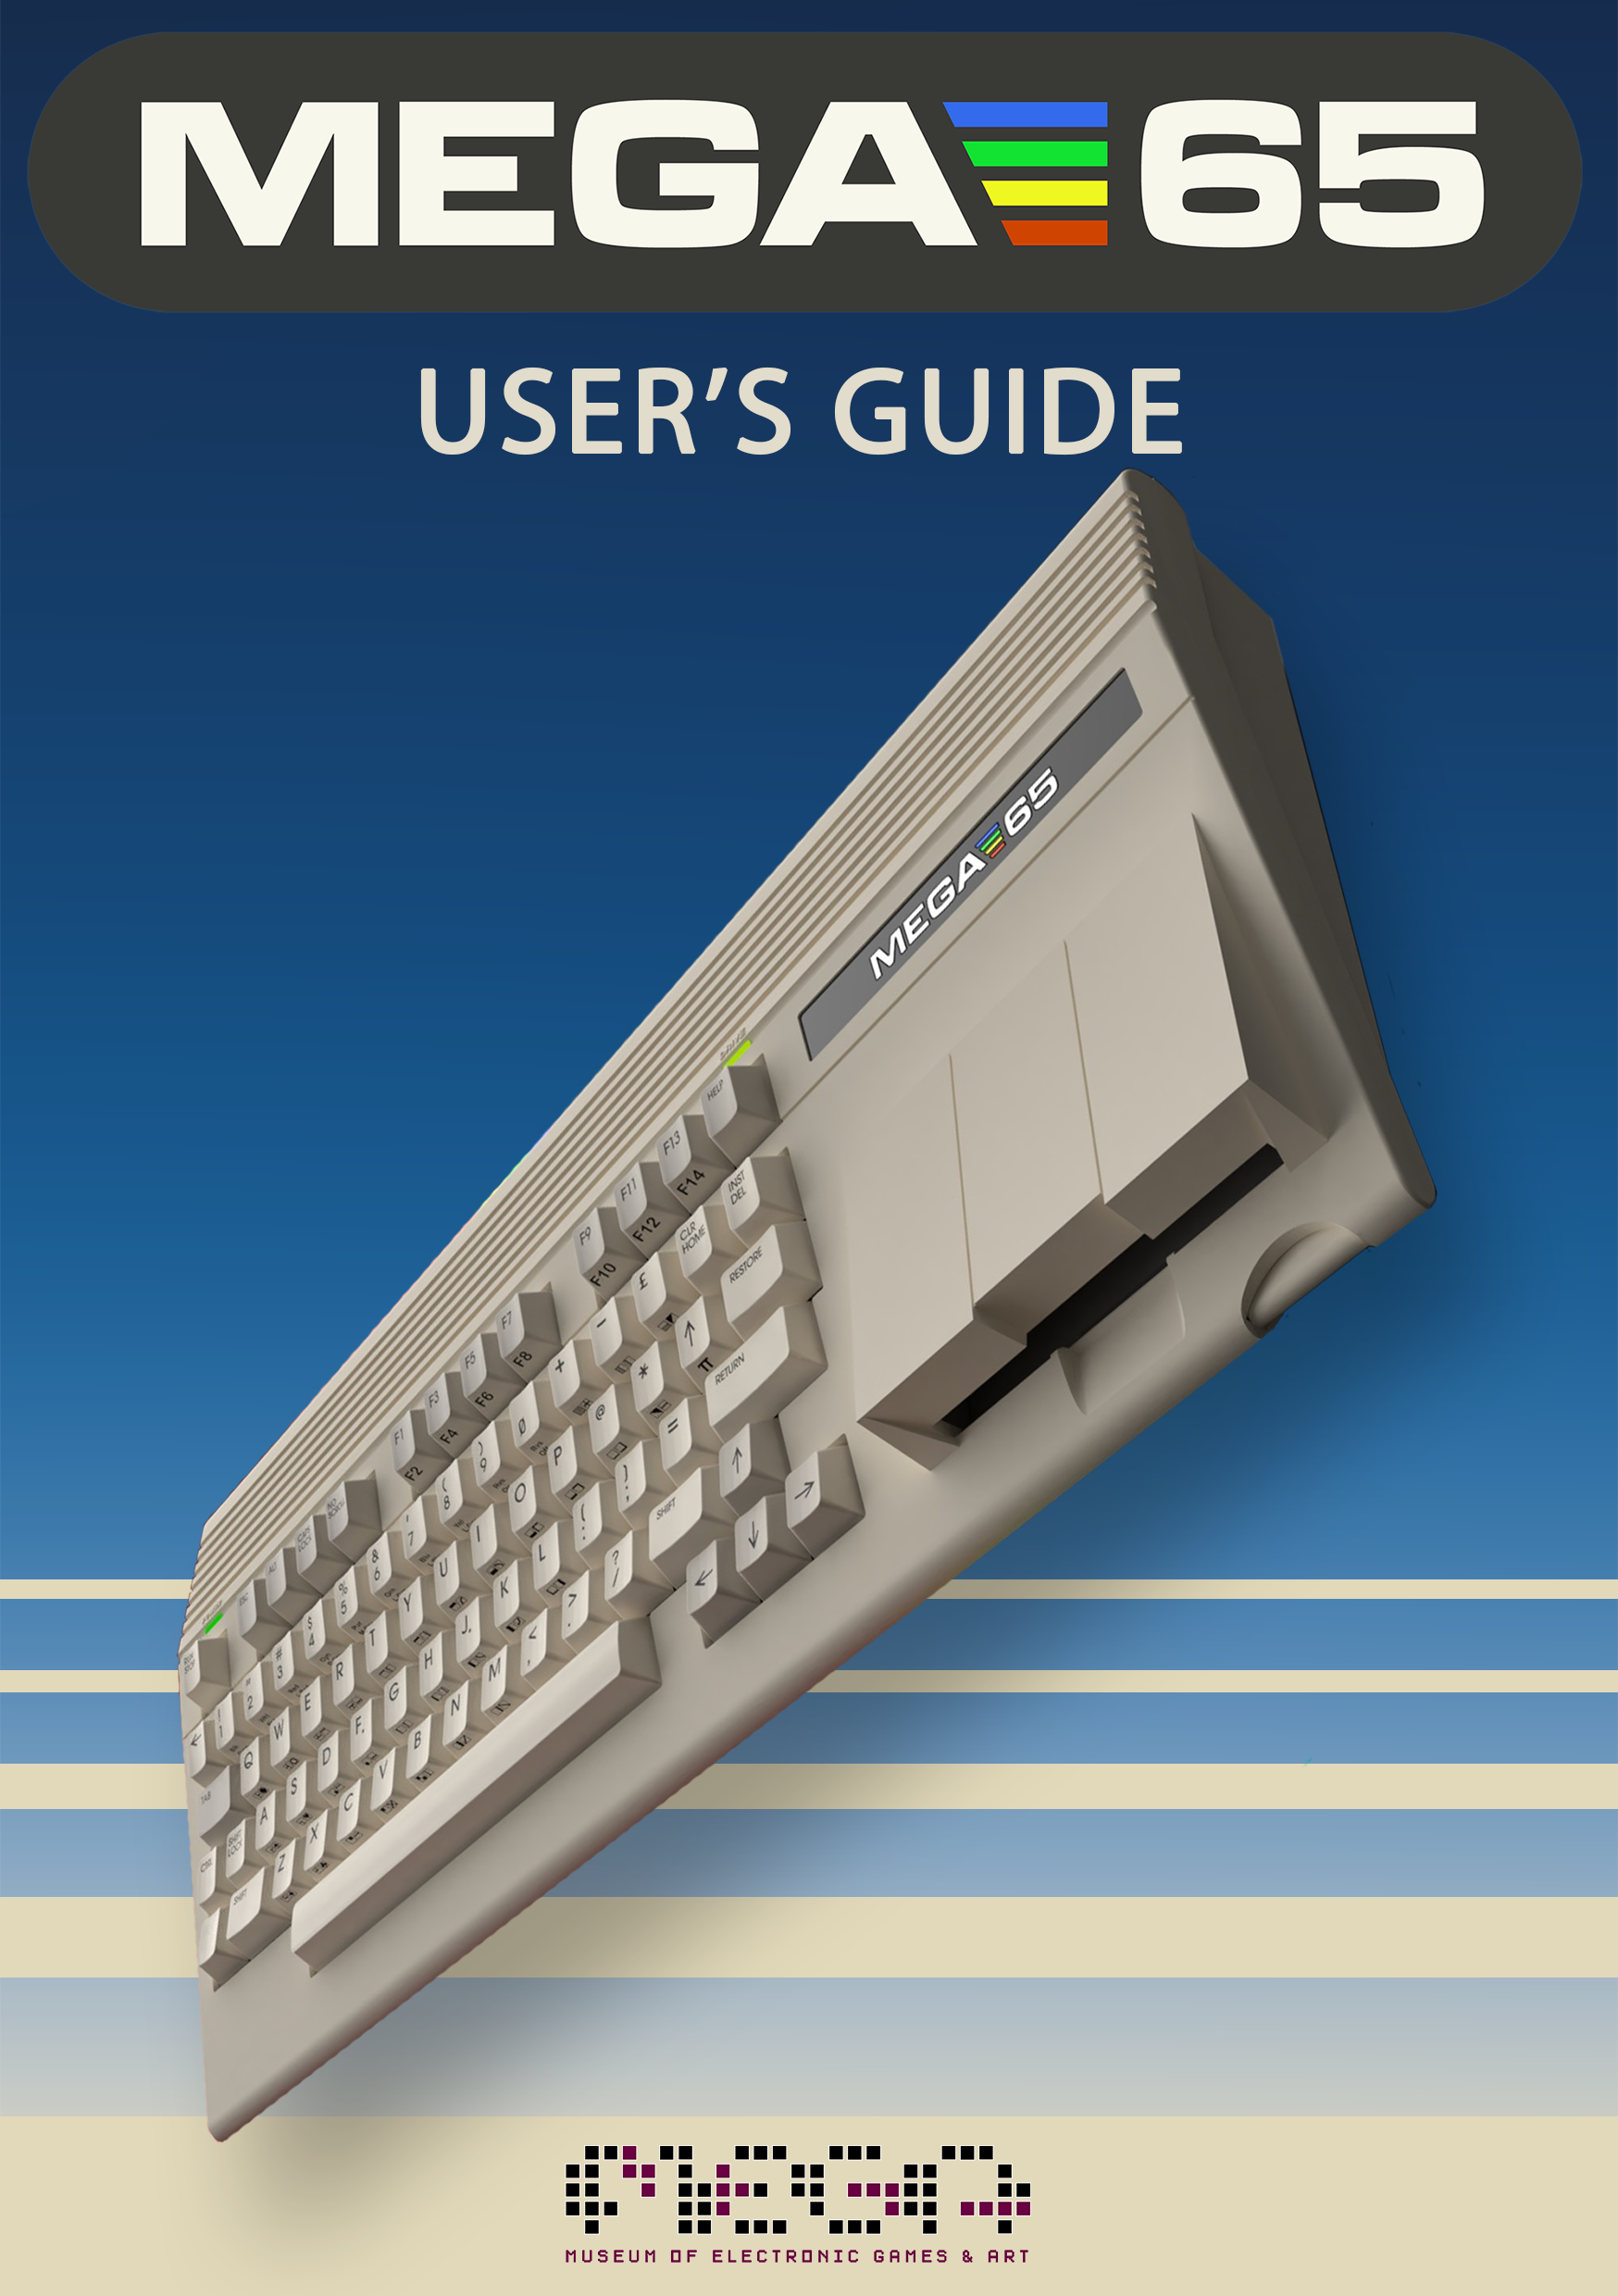
\includegraphics[height=210mm,width=149mm]{frontcover/manual_title}};
\end{tikzpicture}

%\newpage
%\pagecolor{white}


%
% paper title
% Titles are generally capitalized except for words such as a, an, and, as,
% at, but, by, for, in, nor, of, on, or, the, to and up, which are usually
% not capitalized unless they are the first or last word of the title.
% Linebreaks \\ can be used within to get better formatting as desired.
% Do not put math or special symbols in the title.

\cleardoublepage

\pagenumbering{roman}

  \begin{titlepage}
    \pagecolor{blue}
     \begin{center}
       {
         \large
         % Put a nice amount of vertical space before the title
         \vspace*{2cm}
               {\Huge\textcolor{white}{\bf{MEGA65 USER'S GUIDE}}}\\
             \vspace{\fill}
                 {\textcolor{white}{Published by \\ the MEGA Museum of Electronic Games and Art, Germany.\\and\\Flinders University, Australia.}}
       }
     \end{center}
   \end{titlepage}

% Then the copyright notice page
  \pagecolor{white}\textcolor{black}
  \vfill
  WORK IN PROGRESS
  
  \index{copyright}Copyright \copyright 2018 -- 2019 by Paul Gardner-Stephen, Flinders University, the MEGA Museum of Electronic Games and Art, and other contributors.

  This user-guide is made available under the GNU Free Documentation License v1.3, or later, if desired. This means that you are free to modify, reproduce
  and redistribute this user guide, subject to certain conditions. The full text of the GNU Free Documentation License v1.3 can be
  found at \url{https://www.gnu.org/licenses/fdl-1.3.en.html}.

  Implicit in this copyright license, is the permission to duplicate and/or redistribute this document in whole or in part for use in
  education environments.  We want to support the education of future generations, so if you have any worries or concerns, please
  contact us.
             
   \par\today


\pagecolor{white}

%% XXX - big numbers are not in bold, because latex gets confused
\newcommand*{\justifyheading}{\raggedleft}
\definecolor{headingblue}{rgb}{0.5,0.5,1}
\titleformat{\section}[display]{\raggedright}{\thesection}{20pt}{\huge\bf\color{headingblue}\uppercase}[\color{black}]
\titleformat{\chapter}[display]
            {\thispagestyle{empty}\pagecolor{blue}\normalfont\huge\bfseries\justifyheading}
            {\textcolor{white}{\uppercase\chaptertitlename\  {\fontsize{100}{130}\selectfont \bf\thechapter}}}
            {20pt}
            {\Huge\textcolor{white}}[\textcolor{white}{\chapmtoc\insertminitoc}\newpage\newpage\pagecolor{white}\textcolor{black}]
\titleformat{\part}[display]
            {\thispagestyle{empty}\pagecolor{blue}\normalfont\huge\bfseries\justifyheading}
            {\textcolor{white}{\uppercase{\fontsize{50}{65}\selectfont \bf{PART\ }}{\fontsize{100}{130}\selectfont \bf{\serifed\thepart}}}}
            {20pt}
            {\Huge\textcolor{white}}[\textcolor{white}{\partmtoc\insertparttoc}\newpage\newpage\pagecolor{white}\textcolor{black}]
\titlecontents{\chapter}
  
\begin{appendices}

  \chapter{Using a Nexys4DDR as a MEGA65}

\section{Building your own MEGA65 Compatible Computer}

You can build your own MEGA65-compatible computer by using a Nexys4DDR FPGA development board.
This appendix describes the process to setup a Nexys4DDR board for this purpose.
The older non-DDR Nexys4 board is also supported, and the instructions are the same, except that
you must use a bitstream designed for that board.
Using a Nexys4DDR bitstream on a non-DDR Nexys4 board, or vice versa, may cause irrepairable damage to your board, so make sure
you have the correct bitstream to suit your board.


DISCLAIMER: M.E.G.A cannot take any responsibility for any damage that may occur to your Nexys4DDR board.


\section{Power, Jumpers, Switches and Buttons}

The MEGA65 core consumes too much power for the Nexys4DDR board to by powered only from a standard USB port.
In particular, writing to the SD card will hang or do other annoying things.
Therefore you should use a 5V power supply.
Digilent sell a power supply for the Nexys4DDR board, and we recommend you use this to ensure you avoid the risk of damage
to your Nexys4DDR board.

You must then set the following jumpers on your Nexys4DDR board to the following positions:

\begin{itemize}
\item{JP1} - USB/SD
\item{JP2} - SD
\item {JP3} - Wall
\end{itemize}

% XXX - Image of board highlighting the jumpers

All 16 switches on the lower edge of the board must be set to the off position.

The ``CPU RESET'' button will reset the MEGA65 when pressed, while the ``PROG'' button will cause the FPGA itself to reload the MEGA65
core.  The main difference between the two is that CPU RESET is faster, and does not clear the contents of memory, while the FPGA button
is slower, and does reset the contents of memory.

Two of the five buttons in the cross arrangement can also be used:  BTNU acts as though you have pressed the \megakey{RESTORE} key, while BTNC will trigger an IRQ, as though the IRQ line had been pulled to ground.

\section{Keyboard}

Only USB keyboards that lack a USB hub will work with the Nexys4DDR board.  Generally extremely cheap keyboards will work, while more expensive keyboards tend to have a USB hub integrated, and will not work.  You may need to try several keyboards, before you find one that works.

The keyboard layout is positional rather than logical.
This means that keys in similar positions to the keys on a C65 keyboard will have similar function.
This relationship assumes that your USB keyboard uses a US keyboard layout.

The \megakey{RESTORE} key is mapped to the PAGE UP key.

\section{Preparing microSDHC card}

The MEGA65 requires an SDHC card of between 4GB and 64GB capacity.  Some SDXC cards may work, however, this is not officially supported.

To prepare your SD card, you will need the following two separate files from the MEGA65 web site:

\begin{itemize}
\item{Bitstream} \url{http://mega65.org/assets/bitstream.7z}
\item{Support Files} \url{http://mega65.org/assets/fileset.7z}
\end{itemize}

In addition, you will also need a C65 ROM.  There were many different versions created during the development of the Commodore 65,
an the MEGA65 can use any of them.  However, we recommend you use 911001.bin, as this has the most complete BASIC and DOS implementations.

The steps are:

\begin{itemize}
  \item{Format the SD card}  in a convenient computer using the FAT32 filesystem.  The MEGA65 and Nexys4DDR boards do not understand other
file systems, especially the exFAT file system.
\item{Unzip} the bitstream.7z file, and copy the file with name ending in ``.bit'' onto the SD card.
\item{Insert} the SD card into the SD card slot on the under-side of the Nexys4DDR board.
\item{Turn on} the Nexys4DDR board.
\item{Enter the Utility Menu} by holding the left and right SHIFT keys down on the USB keyboard you have connected to the Nexys4DDR board.
\item{Enter the FDISK/FORMAT tool} by pressing 2 when the option appears on the MEGA65 boot screen.
\item{Follow the prompts} in the FDISK/FORMAT program to again format the SD card for use by the MEGA65.
  (The FDISK tool will partition your SD card into two partitions and format them. 
  One is type \$41 = MEGA65 System Partition, where the save slots, configuration data etc. live. 
  (This partition is invisible in i.e. Win PCs).
  and the other partition with type \$0C = VFAT32, where KERNEL,support files, Games, and so on, will be copied to later.
  (This Partition is visible on i.e. Win PCs).
\item{Once formatting is complete} switch off the Nexys4DDR board and remove the microSDHC card from the Nexys Board and put it back into your PC
\item{Again copy} the Bitstream back onto the SD card, as well as all the files from the other 7z file downloaded from the MEGA65 website.
\item{Copy the 911001.bin} ROM file onto the SD card, and rename it to MEGA65.ROM
\item{If you have any .D81 files}, copy them onto the SD card. Make sure that they have names that fit the old DOS 8.3 character limit, and are upper case.  This restriction will be removed in a future release.
\item{Remove the SD card} and reinsert it into your Nexys4DDR board
\item{Power the Nexys4DDR} board back on.  The MEGA65 should boot within 15 seconds.
\end{itemize}


\quote{Congratulations your Mega65 has been set up and is Ready to use !!!}

								 

\section{Useful Tips}

The following are some useful tips for getting familiar with the MEGA65

\begin{itemize}

\item{Press \& hold \megakey{MEGA} (or the \megakey{C=} if using a Commodore 64 or 65 keyboard) during boot to start up in C64 mode instead of C65 mode}
 \item{Press \& hold \megakey{RUN/STOP} during boot to enter the machine language monitor, instead of starting BASIC.}
\item{Press the \megakey{RESTORE} key for approximately 1/2 - 1 second to enter the MEGA65 Freeze Menu.  From this menu
  you have conveient tools to change the CPU speed, switch between PAL \& NTSC video mode, change Audio settings, manage freeze-states,
   select D81 disk images, examine and modify memory of the frozen program, among other features.  This is in many ways the heart of the MEGA65, so it is well worth exploring and familiarising  yourself with!}
\item{Press the \megakey{RESTORE} for about 2 seconds to reset the MEGA65.  This is a temporary feature that will be removed when the MEGA65 desktop computers with built-in reset button become available.}
\item{Type \screentext{POKE0,65} in C64 mode to switch to the CPU to full speed (40MHz). Some software may behave incorrectly in this mode, while other software will work very well, and run many times faster than on a C64.}
\item{Type \screentext{POKE0,64} in C64 mode to switch the CPU to 1MHz.}
\item{Type \screentext{SYS58552} in C64 mode to switch to C65 mode.}
\item{Type \screentext{GO64} in C65 mode and confirm, by pressing \screentext{Y}, to switch to C64 mode, just like on a C128.}
\item{The C65 ROM makes device 8 the default, so you can normally leave off the ,8 from the end of LOAD and SAVE commands.}
\item{Pressing \megakey{SHIFT} + \megakey{RUN/STOP} from either C64 or C65 mode will attempt to boot from disk.}
\item{Have fun! The MEGA65 has been loving crafted over many years for your enjoyment. We hope you have as much fun using it, as we have had creating it!}
\item{The MEGA Museum of Electronic Games and Art welcomes your feedback, suggestions and contributions to this open-source digital heritage preservation project.}
\end{itemize}


\end{appendices}



\bibliographystyle{IEEEtran}
\bibliography{references}

\end{document}

